\title[TOF QA]{ {\Huge TOF QA report} } % The short title appears at the bottom of every slide, the full title is only on the title page
\subtitle{\Large Data period -- {{ periodname }} {{ passname }} } % The short title appears at the bottom of every slide, the full title is only on the title page

\author[ {{ presenter }}]{
  {{ authors }}\\
  on behalf of the TOF group
} % Your name



\titlegraphic{
  
\includegraphics[width = \textwidth, keepaspectratio=true]{images/4_Color_Logo_CB.png}
}
\institute[ {{ presenterinstitute }} ] % Your institution as it will appear on the bottom of every slide, may be shorthand to save space
{
  {
      \tiny
      {{ institutes }}
    }
  \\
  \medskip

  {
    \large
    QA meeting -- \today
  }

  \medskip

}


{
  \centering
  \usebackgroundtemplate{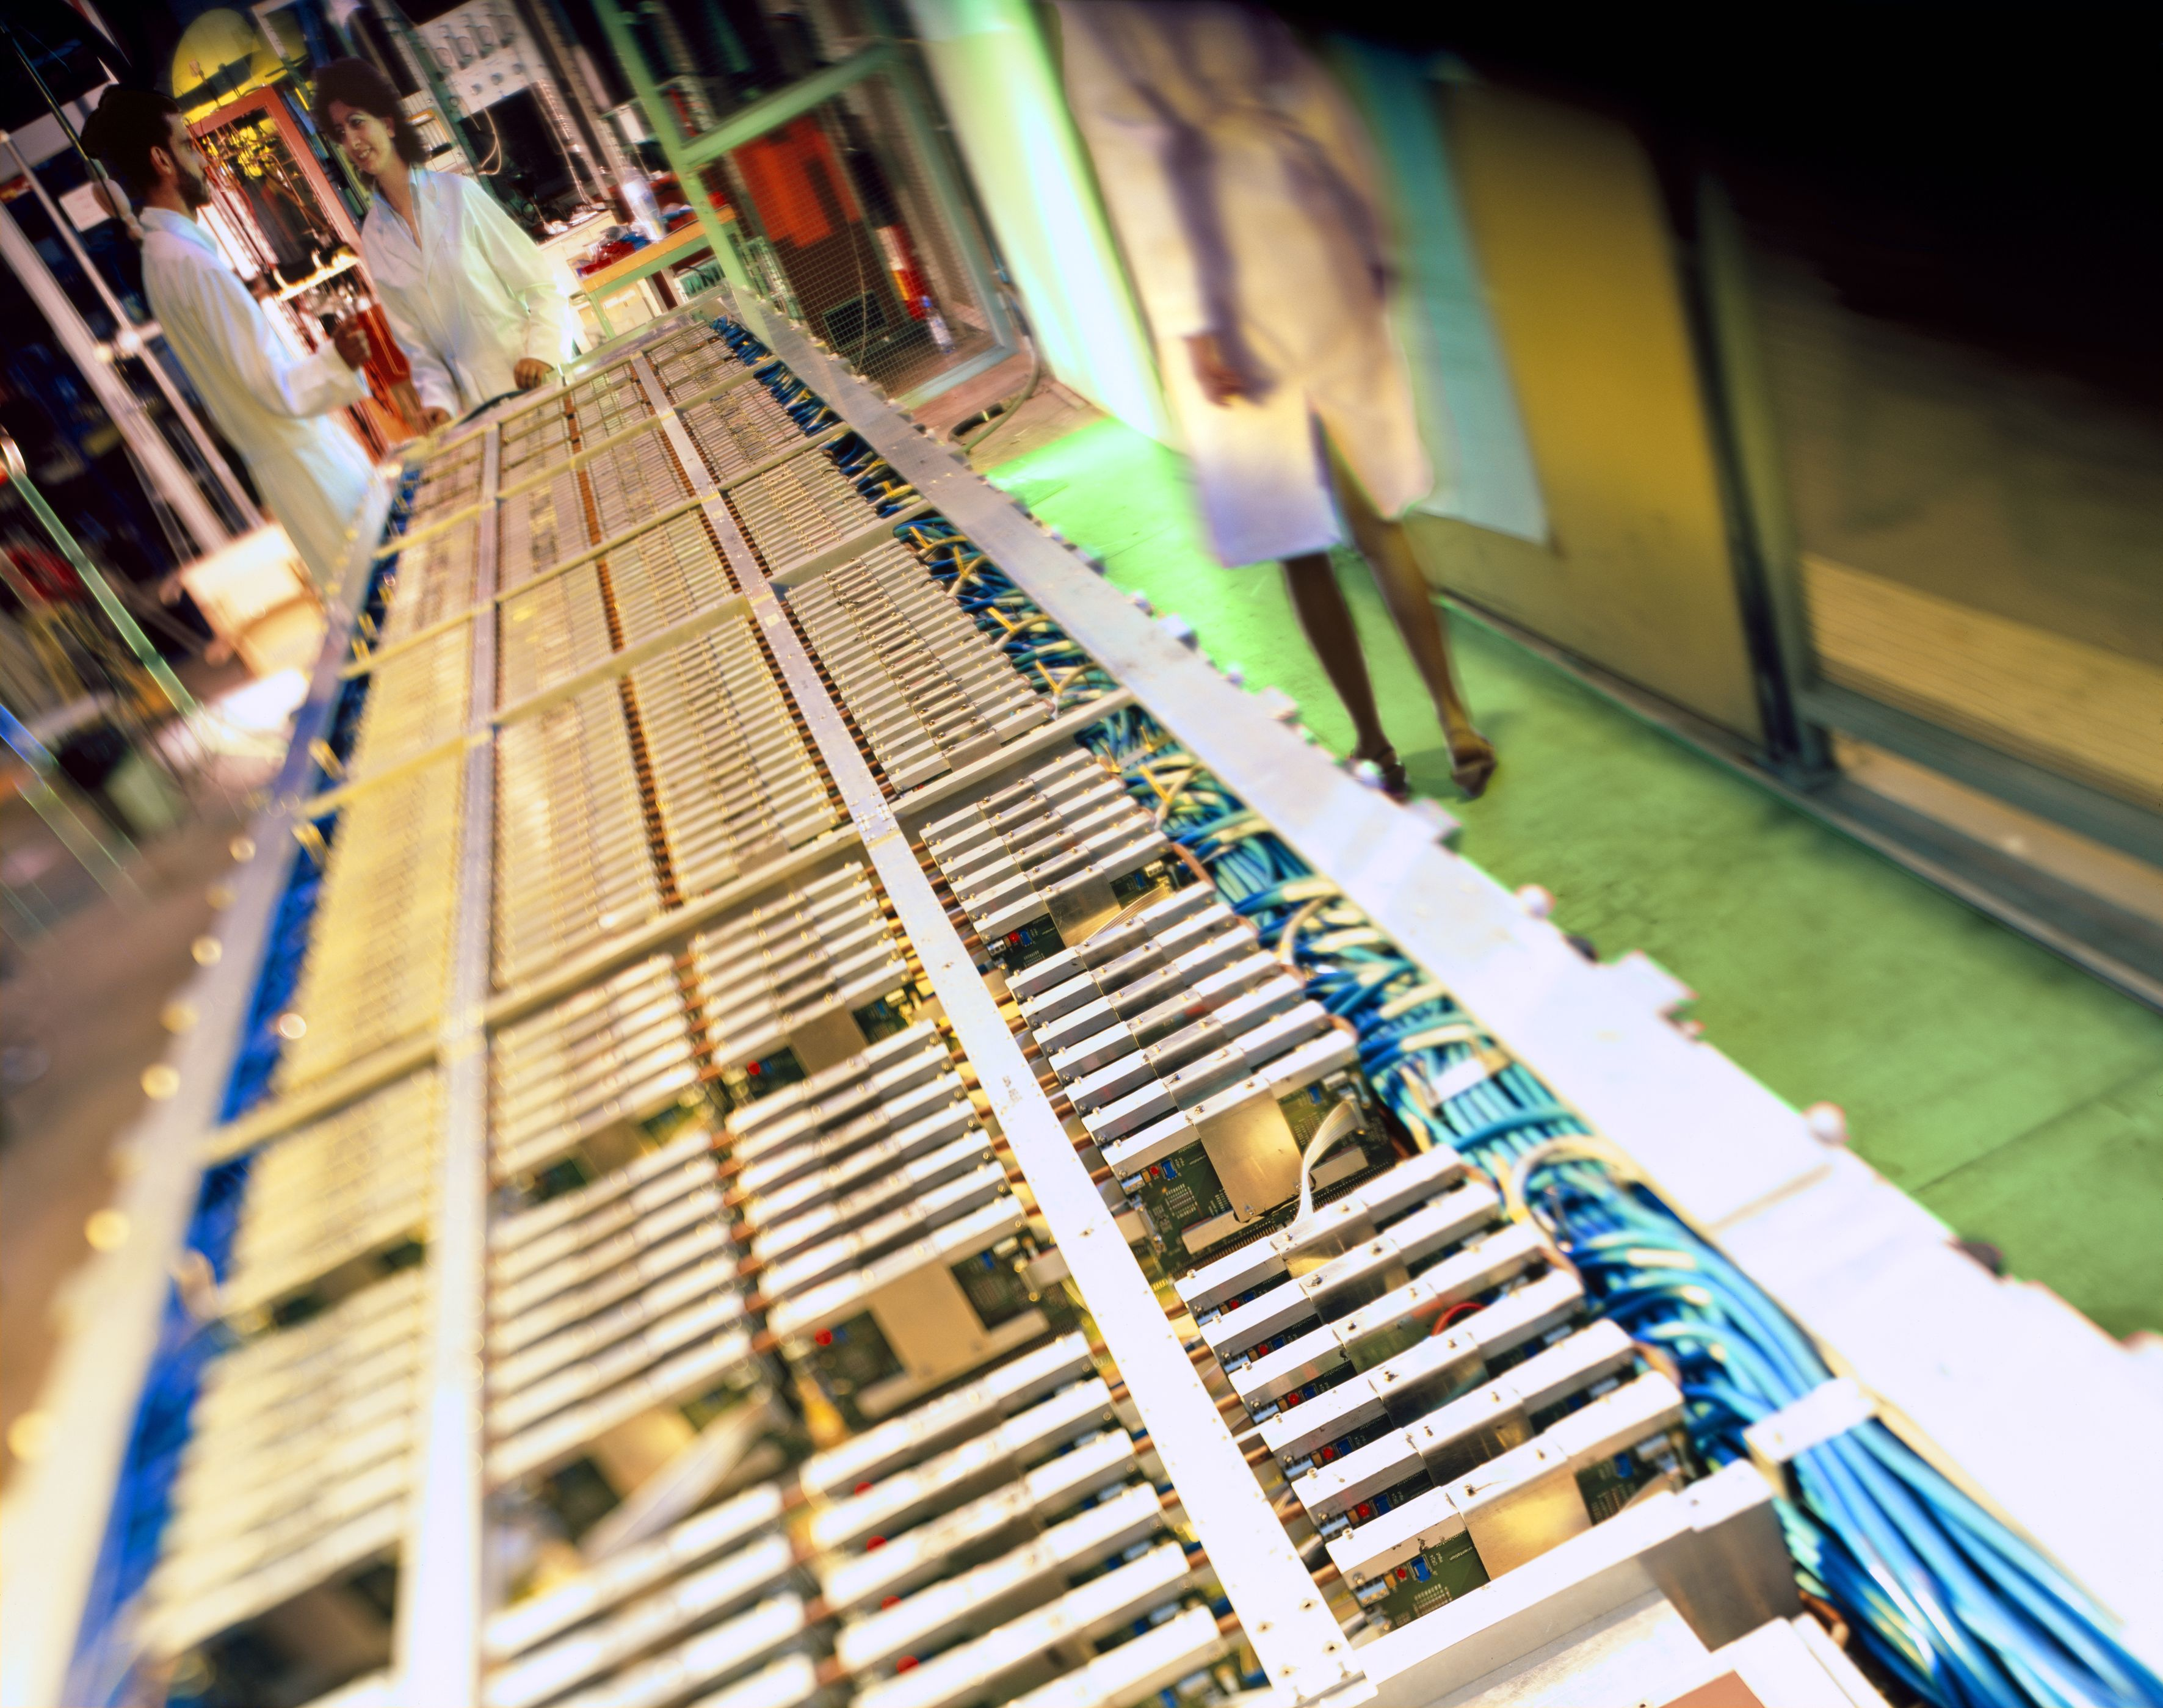
\includegraphics[trim = 0 0 0 300, clip,width=\paperwidth,keepaspectratio]{images/tof-2006-011}}
  \begin{frame}
    \maketitle
  \end{frame}
}
